\chapter{Discrete Fourier Transform}

The Discrete Fourier Transform or DFT is the Fourier Transform of a finite length DT signal. As we shall see, the DFT/FFT is mathematically equivalent to the Discrete-Time Fourier Series. It can be viewed as a way to numerically approximate the CT Fourier transform. Lets first just state the transform and then derive it and see how to interpret and apply it.

Given a finite-length sequence of real or complex numbers $x[n]$, indexed from $0$ to $N-1$, the \emph{Discrete Fourier Transform} or DFT is given by
\[
X[k] = \sum_{n = 0}^{N-1}  x[n] e^{-j \frac{2\pi}{N}k n}
\]
for $k = 0, 1, 2, \cdots, N-1$. When $N$ is a power of 2, an efficient algorithm to compute this result exists and is called the \emph{Fast Fourier Transform} or FFT.

\section{Numerically Approximating the CT Fourier Transform}

Recall the CT Fourier transform pair $x(t) \stackrel{\mathcal{F}}{\longleftrightarrow} X(j\omega)$:
\[
X(j\omega) = \int\limits_{-\infty}^{\infty} x(t) e^{-j\omega t} \; dt
\]

\[
x(t) = \frac{1}{2\pi} \int\limits_{-\infty}^{\infty} X(j\omega) e^{j\omega t} \; d\omega
\]

How could we compute these when we have a physical signal, rather than just a mathematical model?

Recall from calculus the (left) Riemann sum approximation of a definite integral
\[
\int\limits_{t_1}^{t_2} f(t) \; dt = \lim_{N \rightarrow \infty} \sum_{n = 0}^{N-1} \frac{t_2-t_1}{N} f\left(t_1 + n\frac{t_2-t_1}{N}\right) 
\]
\begin{center}
  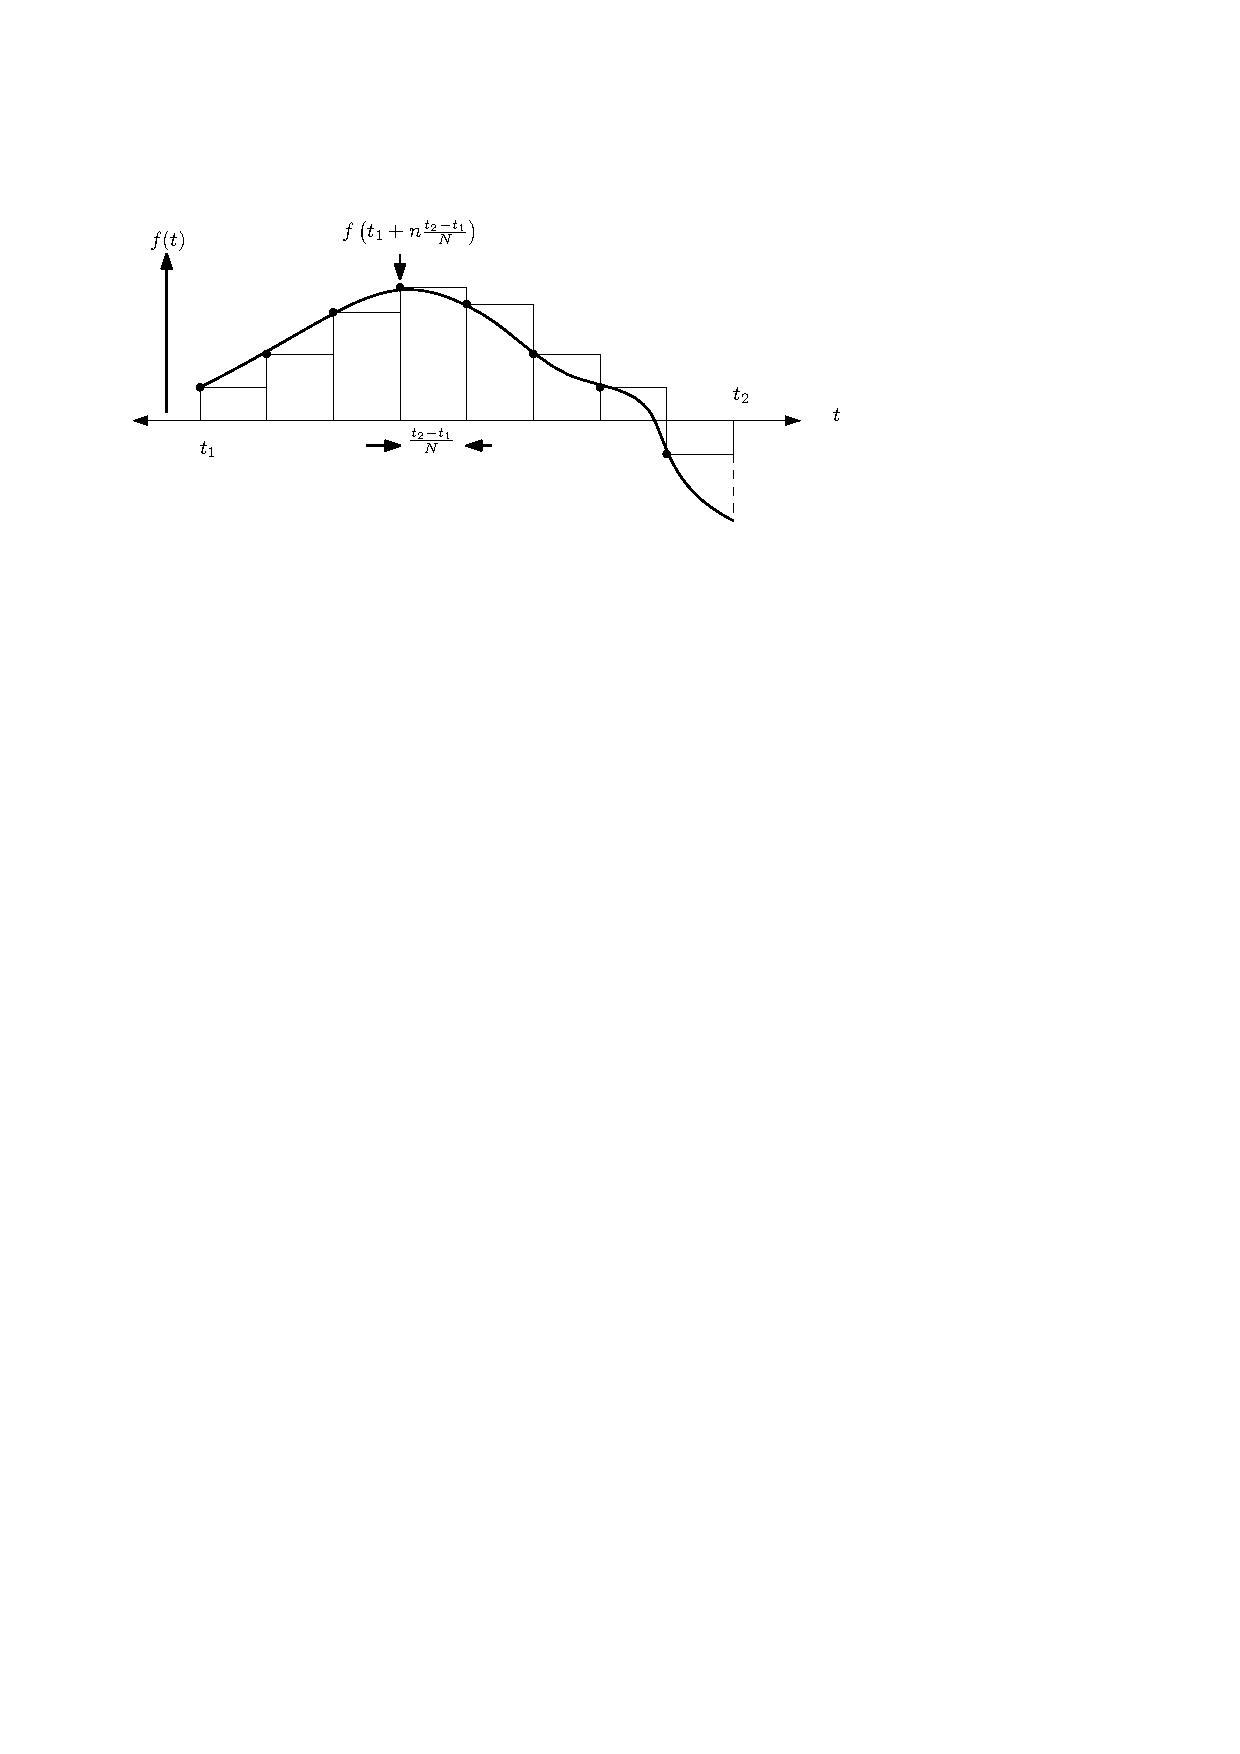
\includegraphics[scale=0.9]{graphics/riemann_sum.pdf}
\end{center}
In the case of the CTFT, if the signal $x(t)$ is non-zero only over some interval $(t_1, t_2)$, then
\[
\mathcal{F}\{ x(t) \} = \int\limits_{t_1}^{t_2} x(t) e^{-j\omega t} \; dt \approx \sum_{n = 0}^{N-1} \frac{t_2-t_1}{N} x\left(t_1 + n\frac{t_2-t_1}{N}\right) e^{-j\omega \left(t_1 + n\frac{t_2-t_1}{N}\right)} 
\]
for large $N$.\\[1em]

If we define the time sample spacing as $T = \frac{t_2-t_1}{N}$, then
\[
X(j\omega) \approx \sum_{n = 0}^{N-1} T \, x\left(t_1 + nT\right) e^{-j\omega \left(t_1 + nT\right)}
\]

Note $x\left(t_1 + nT\right)$ corresponds to \emph{samples} of $x(t)$ starting at $t_1$ with sampling interval $T$. This information is equivalent to the triad $t_1, T, x[n]$, where $x[n]$ is a finite length sequence of numbers, i.e. a DT signal where $x[n] = 0$ for $n < 0$ and $n \geq N$. Thus,

\[
x\left(t_1 + nT\right) = x[n]
\]

Substituting into our approximation
\[
X(j\omega) \approx \sum_{n = 0}^{N-1} T \, x\left(t_1 + nT\right) e^{-j\omega \left(t_1 + nT\right)} = T e^{-j\omega t_1} \sum_{n = 0}^{N-1} x[n] e^{-j\omega n T} 
\]

Now, consider a sampling of the frequency axis $\omega = \frac{2\pi}{NT} k$. Then
\[
\omega n T = \frac{2\pi}{N T} k n T = \frac{2\pi}{N}k n
\]
and
\[
X\left(j\frac{2\pi}{NT} k\right) = T e^{-j\omega t_1} \underbrace{\sum_{n = 0}^{N-1} x[n]  e^{-j \frac{2\pi}{N}k n}}_{\text{DFT}} = T e^{-j\omega t_1} \, X[k] 
\]

Thus we see the DFT corresponds to the Fourier transform of a sampled CT signal over a limited time-interval, at samples of the frequency axis.

Similarly, in the case of the Inverse CTFT, if the signal $X(j\omega)$ is non-zero only over some interval $(\omega_1, \omega_2)$, then
\begin{align*}
  \mathcal{F}^{-1}\{ X(j\omega) \} &= \frac{1}{2\pi} \int\limits_{\omega_1}^{\omega_2} X(j\omega) e^{j\omega t} \; dt\\ &\approx \frac{1}{2\pi} \sum_{k = 0}^{M-1} \frac{\omega_2-\omega_1}{M} X\left(\omega_1 + k\frac{\omega_2-\omega_1}{M}\right) e^{j \left(\omega_1 + k\frac{\omega_2-\omega_1}{M}\right)t} 
\end{align*}
for large $M$. If we define the frequency sample spacing as $W = \frac{\omega_2-\omega_1}{M}$, then
\[
x(t) \approx \sum_{m = 0}^{M-1} \frac{W}{2\pi}  \, X\left(\omega_1 + kW\right) e^{j\left(\omega_1 + kW\right)t}
\]

Note $X\left(\omega_1 + mW\right)$ corresponds to samples of $X(j\omega)$ starting a $\omega_1$ with sampling interval $W$. This information is equivalent to the triad $\omega_1$, $W$, $X[k]$, where $X[k]$ is a finite length sequence of numbers where 
\[
X\left(\omega_1 + mW\right) = X[k]
\]
Substituting 
\[
x(t) \approx \sum_{m = 0}^{M-1} \frac{W}{2\pi}  \, X\left(\omega_1 + kW\right) e^{j\left(\omega_1 + kW\right)t} = \frac{W}{2\pi} e^{j\omega_1} \sum_{m = 0}^{M-1}  X[k] e^{j kWt} 
\]

Consider the sampling of the time axis in the derivation of the DFT, $t = nT$. Let $\omega_1 = 0$ and $\omega_2 = \frac{2\pi}{T}$ and $M = N$. Then
\[
kWt = kWnT = k \frac{2\pi}{NT} n T = \frac{2\pi}{N}kn
\]
Since $W = \frac{2\pi}{NT}$
\[
x(nT) = \frac{1}{T} \underbrace{\frac{1}{N} \sum_{k = 0}^{N-1}  X[k] e^{j \frac{2\pi}{N}k n}}_{\text{Inverse DFT}} = \frac{1}{T} x[n] 
\]
Thus we see the IDFT corresponds to the Inverse Fourier transform of a sampled Fourier Transform over a limited bandwidth, at samples of the time axis.

This gives us the DFT pair
\[
X[k] = \text{DFT} \{ x[n] \} = \sum_{n = 0}^{N-1}  x[n] e^{-j \frac{2\pi}{N}k n}
\]
\[
x[n] = \text{IDFT} \{ x[n] \} = \frac{1}{N} \sum_{k = 0}^{N-1}  X[k] e^{j \frac{2\pi}{N}k n}
\]
Note the similarity to the DT Fourier Series when $N_0 = 0$
\[
x[n] = \sum\limits_{k = N_0}^{N_0 + N - 1} a_k e^{j\frac{2\pi}{N}kn} =  \sum\limits_{k = 0}^{N - 1} a_k e^{j\frac{2\pi}{N}kn}
\]
\[
a_k = \frac{1}{N}\sum\limits_{n = N_0}^{N_0 + N - 1} x[n] e^{-j\frac{2\pi}{N}kn} =  \frac{1}{N}\sum\limits_{n = 0}^{N - 1} x[n] e^{-j\frac{2\pi}{N}kn}
\]

\section{Efficient Computation of DFT (FFT)}

Given the DFT pair and an input signal, it is easy to compute the DFT. For example in C++ we can define a signal as an array of complex numbers

\begin{verbatim}
#include <complex>
#include <vector>

typedef Signal std::vector<std::complex<double>>;
\end{verbatim}

and implement the DFT in a straightforward translation of the expressions above:

\begin{verbatim}
Signal dft(const Signal & in){

  Signal out = in;
  
  const int N = in.size();

  for(int k = 0; k < N; ++k){
    out[k] = 0;
    for(int n = 0; n < N; ++n){
      out[k] += in[n]*exp(-j*2.*PI*double(k)*double(n)/double(N));
    }
  }

  return out;
}
\end{verbatim}

Because of the nested for loops the number of multiplies and adds required to compute the DFT is proportional to the number of samples in the signal, squared. However, by expanding the complex exponential we see
\begin{align*}
  X[k] &= \sum_{n = 0}^{N-1}  x[n] e^{-j \frac{2\pi}{N}k n}\\
  &= \sum_{n = 0}^{N-1}  x[n] \left\{ \cos\left( -\frac{2\pi}{N}k n\right) + j \sin\left(-\frac{2\pi}{N}k n \right)\right\}\\
  &= \sum_{n = 0}^{N-1}  x[n] \left\{ \cos\left( \frac{2\pi}{N}k n\right) - j \sin\left(\frac{2\pi}{N}k n \right)\right\}
\end{align*}
Which can be compactly written as
\[
X = \mathcal{W} x
\]
where $x \in \mathbb{C}^N$ is the sampled signal treated as a complex-valued vector, and $\mathcal{W} \in \mathbb{C}^{N\times N}$ is a complex-valued matrix with entries
\[
\mathcal{W}_{k\,n} = \cos\left( \frac{2\pi}{N}k n\right) - j \sin\left(\frac{2\pi}{N}k n \right) = \left( e^{-j\frac{2\pi}{N}}\right)^{kn}
\]  

Similarly for the inverse DFT
\begin{align*}
  x[n] &= \sum_{k = 0}^{N-1}  X[k] e^{j \frac{2\pi}{N}k n}\\
  &= \sum_{k = 0}^{N-1}  X[k] \left\{ \cos\left( \frac{2\pi}{N}k n\right) + j \sin\left(\frac{2\pi}{N}k n \right)\right\}
\end{align*}
Which can be compactly written as
\[
x = \frac{1}{N} \mathcal{W}^{*} X
\]

This implies $\frac{1}{N}\mathcal{W}\mathcal{W}^* = I$. This special structure ($\mathcal{W}$ is orthogonal) is what enables the Fast Fourier Transform algorithm to compute the DFT/IDFT in $O(N\log_2 N)$ multiply/adds. The most common algorithm for implemeting the FFT is called the Cooley–Tukey radix-2 algorithm. This algorithm can be implemented using C++ as:

\begin{verbatim}
Signal fft(const Signal & in){

  Signal out;

  std::size_t n = in.size();
  double logn = log2(n);

  for (unsigned int i = 0; i < n; ++i) {
    int rev = bitReverse(i, logn);
    out[i] = in[rev];
  }

  // make sure logn is positive integer > 1
  std::size_t temp = static_cast<std::size_t>(logn);
  assert(static_cast<double>(temp) == logn);

  for(std::size_t s = 1; s <= logn; ++s){
    std::complex<double> w(1,0);

    int m = 1 << s; // 2 power s
    int m2 = m >> 1; // m2 = m/2 -1

    std::complex<double> wm = exp(-PI*j/static_cast<double>(m2));

    for(std::size_t j = 0; j < m2; ++j){
      for(std::size_t k = j; k < n; k+=m){
        std::complex<double> t = w*out[k+m2];
        std::complex<double> u = out[k];
        out[k] = u + t;
        out[k+m2] = u - t;
      }
      w = w*wm;
    }
  }

  return out;
}
\end{verbatim}

where the function \texttt{bitReverse} reverses the bitwise representation of the index argument

\begin{verbatim}
unsigned int bitReverse(unsigned int x, int log2n){
  int n = 0;
  for (int i = 0; i < log2n; i++){
    n <<= 1;
    n |= (x & 1);
    x >>= 1;
  }
 return n;
}
\end{verbatim}

\section{DFT/FFT in Matlab}

In Matlab (and other languages/platforms) you can use the Fast Fourier Transform to compute the DFT. For example:

\begin{verbatim}
>> T = 0.001;
>> t = 0:T:100;
>> x = cos(2*pi*t);
>> X = fft(x);
>> plot(abs(X))
\end{verbatim}
To give a plot consistent with the CTFT
\begin{verbatim}
>> w = (-pi/0.001):(2*pi/100):(pi/0.001);
>> stem(w, T*fftshift(abs(X)))
\end{verbatim}
or
\begin{verbatim}
>> stem(w, T*fftshift(angle(X)))
\end{verbatim}


\section{Summary of Fourier Transforms}

\begin{itemize}
\item Discrete-time Fourier Series: periodic DT signal $x[n] \mapsto a_k$ periodic discrete frequencies
\item Discrete-time Fourier Transform: aperiodic DT signal of indefinite length $x[n] \mapsto X(e^{j\omega})$ periodic continuous frequencies
\item Continuous-time Fourier Series: periodic CT signal  $x(t) \mapsto a_k$ discrete frequencies of indefinite length
\item Continuous-time Fourier Transform: aperiodic CT signal of indefinite length  $x(t) \mapsto X(j\omega)$ continuous frequencies 
\end{itemize}

And now we have the DFT
\begin{itemize}
\item Discrete Fourier Transform: aperiodic DT signal of finite length $x[n] \mapsto X[k]$ periodic discrete frequencies
\end{itemize}

\section{Applications the DFT}

Our discussion of the DFT raises some important questions:

\begin{itemize}
\item For what values of sampling interval $T$ does this hold?
\item What are the effects of time and frequency sampling on $x(t)$ and $X(j\omega)$?
\item What if $x(t)$ or $X(j\omega)$ is non-zero outside the interval?
\end{itemize}
These will be answered in the last two lectures. It also admits some important applications:
\begin{itemize}
\item Numerical computation of Fourier transform of physical signals
\item Simulation or approximation of stable CT systems
\item Implementation of CT systems using DT systems
\end{itemize}

As an example application, suppose you have a physical signal, say an audio signal from a microphone. How would you estimate it's Fourier Transform? Sample $x(t)$ at a frequency of $\frac{2\pi}{T}$ for $NT$ seconds.
\[
x[n] = x(nT)
\]
\[
X[k] = \text{DFT}\left\{ x[n] \right\}
\]
\[
X\left(j\frac{2\pi}{NT} k\right) = T X[k]
\]
Note, in practice this requires multiplication by a windowing function to get good results unless there is silence on either side of the audio.

\begin{example}
  Consider a CT signal $x(t) = \cos(2\pi t)\left[u(t) - u(t-100)\right]$ sampled at a frequency of $\frac{2\pi}{0.001}$ for $NT = 100$ seconds to obtain $x[n]$. Given the DFT of $x[n]$, $X[k]$, what values of $k$ correspond to $\omega = \pm 2\pi$?
  
  \[
  \omega = 2\pi = \frac{2\pi}{NT} k \implies k = 100
  \]
  
  \[
  \omega = - 2\pi = \frac{2\pi}{NT} k \implies k = -100
  \]
  However $k \in (0, N-1)$ where $N= 100000$. Thus $k = -100 = N - 100 = 99900$. Note, the Matlab command \texttt{fftshift} does this unwrapping for you.
\end{example}

As another application, suppose you have a CT frequency response, for example a CT filter. How could you simulate the response to a physical signal, such as an audio signal from a microphone? Again, sample $x(t)$ at a frequency of $\frac{2\pi}{T}$ for $NT$ seconds.
\[
x[n] = x(nT)
\]
\[
X[k] = \text{DFT}\left\{ x[n] \right\}
\]
Using the convolution property of the CTFT
\[
Y[k] = H\left(j\frac{2\pi}{NT} k\right) X[k]
\]
\[
y(nT) = \frac{1}{T} \text{IDFT}\left\{ Y[k] \right\}
\]

As a final application example we consider the case of filtering. DT implementations of CT systems have a number of benefits over CT implementations. The previous application hints at a method to implement a CT system using a DFT. We sample $x(t)$ at a frequency of $\frac{2\pi}{T}$ for $NT$ seconds into a buffer, called a \emph{frame}.
\[
x[n] = x(nT)
\]
\[
X[k] = \text{DFT}\left\{ x[n] \right\}
\]
\[
Y[k] = H\left(e^{j\frac{2\pi}{NT} k}\right) X[k]
\]
\[
y(t) \approx y(nT) = \frac{1}{T} \text{IDFT}\left\{ Y[k] \right\}
\]
This last step is called \emph{reconstruction}. Note this can be done in real time using three frames, one being sampled, one being processing, and one being reconstructed.

Note the DT filter in the previous application adds a two frame delay. This delay can be removed using an FIR or IIR filter implementation, as we saw in lecture 25. We can sample $x(t)$ at a frequency of $\frac{2\pi}{T}$ continuously into a \emph{ring buffer}.
\[
x[n] = x(nT)
\]
Compute $y[n]$ using a delay difference equation, e.g. for second order
\[
y[n] = a_1 y[n-2] + a_2 y[n-1] + a_3 x[n-2] + a_4 x[n-1] + a_5 x[n]
\]
Reconstruct the current output
\[
y(t) \approx y(nT) = y[n]
\]

